\chapter{Implementation of Validation Features}
\label{chap:appendixval}

%##################################################################################################
\section{Drawing Tools}
%##################################################################################################

%---
\stufigex{height=10cm}{appendixval/appendixval-pen-closeup.png}{A close-up view of a Bamboo Fun pen tablet and accompanying pen}{fig:appendixval-pen-closeup}{p}
%---

\noindent In order to allow `gold standard' reference segmentations to be produced for validation purposes, it was necessary both to find suitable user input hardware and to implement software tools in \emph{millipede} to allow the user to manually draw round features of interest in 2D slices. The hardware chosen (primarily because I owned one) was a Bamboo Fun pen tablet (manufactured by Wacom) -- see Figure~\ref{fig:appendixval-pen-closeup}. For our purposes here, however, I will focus only on the drawing tools I implemented in my software. Each tool can be used to replace the current selection, augment it (if the \emph{Shift} key is pressed) or subtract from it (if the \emph{Ctrl} key is pressed). Tools were classified as belonging to one of three types:
%
\begin{enumerate}
\item \emph{Instantaneous} tools, where the user clicks a point on the canvas and the selection is immediately updated (e.g.~the type of magic wand tool found in common image-editing programs).
\item \emph{Click-and-drag} tools, where the user clicks a point on the canvas, drags the mouse and then releases it to update the selection.
\item \emph{Multi-click} tools, where the user clicks a number of points and then `finalizes' the selection when ready.
\end{enumerate}

\noindent Three tools were implemented in \emph{millipede} (but it would be easy to add further tools if desired):

\begin{enumerate}

\item A click-and-drag \emph{box} tool. An example use of this is to restrict a 3D selection to a particular axial slice -- this involves switching to coronal or sagittal view and drawing boxes to remove the pieces of selection above and below the desired slice.

\item A click-and-drag \emph{lasso} tool. This can be used to draw round the exact contours of specific features, although it can require a relatively steady hand. If mistakes are made, they can be corrected fairly easily by augmenting/subtracting from the initial selection using further lassoing.

\item A multi-click \emph{line loop} tool. This involves placing a series of points to form a line loop, and then finalizing the result. Previously placed points can be dragged to new positions if mistakes are made. The line loop tool produces results that are less precise than those produced by the lasso, but it is somewhat easier to control.

\end{enumerate}
%
No instantaneous tool was implemented, because it was not essential for validation purposes, but an instantaneous magic wand tool (essentially just a single-click region growing tool) is an obvious candidate for future inclusion. A tool is implemented as a C++ class deriving from the \texttt{DrawingTool} base class shown in Listing~\ref{code:appendixval-drawingtool}. The key things to specify are:

\begin{itemize}

\item How to check whether the user is currently drawing with the tool.
\item What to do when the user presses, drags or releases the mouse. (Note from the listing that the position of the mouse when the user does any of these things is passed to the tool both in on-screen pixel coordinates and in image volume coordinates -- this will be discussed further when talking about partition forest selections later, but the essential point is that rendering is done in pixel coordinates, whereas selections must be created in image volume coordinates. Trying to produce selections by rasterizing in pixel coordinates can produce results that contain holes.)
\item How to render what is currently being drawn.
\item How to reset the tool.
\item How to evaluate the user's input to produce a selection of voxels in the image volume.
\item What style of tool this is.

\end{itemize}
%
Each of the three implemented tools is described below, after which it will be shown how they were actually used to create partition forest selections in \emph{millipede}. It should be noted that the lasso and line loop have a great deal in common, in that both create polylines that must be evaluated to produce a selection of voxels in the image volume (in the lasso case, these are large polylines that are evaluated as soon as the user releases the mouse button; in the line loop case, these are generally small polylines that are evaluated when the user requests it). The evaluation in both cases requires \emph{polyline rasterization}, which will be discussed first. In the code, both tools are implemented as subclasses of a \texttt{LineBasedDrawingTool} class, which maintains the polyline that will ultimately be fed to the rasterizer.

%---
\begin{stulisting}[p]
\caption{The DrawingTool class}
\label{code:appendixval-drawingtool}
\lstinputlisting[style=Default,language=C++]{appendixval/appendixval-drawingtool.lst}
\end{stulisting}
%---

\newpage

%################################################
\subsection{Box Tool}
%################################################

The box tool is relatively straightforward to implement, as shown in Listing~\ref{code:appendixval-boxdrawingtool}. Two points are maintained to represent the extents of the box: an \emph{anchor} point and an \emph{other} point. When drawing a box, the user first presses the mouse: this initialises both points to the position of the mouse press. The user then drags the mouse, which moves the \emph{other} point away from the \emph{anchor} to make the box (see Figure~\ref{fig:appendixval-boxtool}(a)). Finally, the user releases the mouse; since the tool is not of the multi-click variety, this results in \texttt{BoxDrawingTool::selected_positions()} being called to evaluate the actual voxels contained within the box. These are initially in 2D (since the drawing tools are designed as an independent package that doesn't know about the 3D image volume), but are subsequently converted into 3D based on the slice being viewed, and used to construct a partition forest selection (see Figure~\ref{fig:appendixval-boxtool}(b)). The details of this will be described in \S\ref{subsec:appendixval-integration}. Actually determining which voxels are in the box is a trivial process: all that is required is to traverse the box from one of its corners to the other in the obvious manner.

%---
\begin{stusubfig}{h}
	\subfigure[Before evaluating the selection]
	{\hspace{8mm}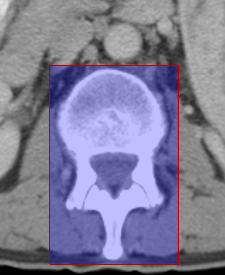
\includegraphics[height=6cm]{appendixval/appendixval-boxtool-before.png}\hspace{8mm}}%
	%
	\hspace{4mm}%
	%
	\subfigure[After evaluating the selection]
	{\hspace{8mm}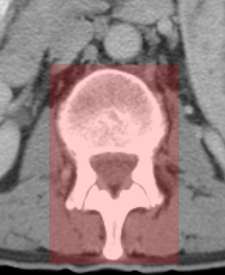
\includegraphics[height=6cm]{appendixval/appendixval-boxtool-after.png}\hspace{8mm}}%
\caption{The box tool being used to select a region containing the spine}
\label{fig:appendixval-boxtool}
\end{stusubfig}
%---

%---
\begin{stulisting}[p]
\caption{The BoxDrawingTool class}
\label{code:appendixval-boxdrawingtool}
\lstinputlisting[style=Default,language=C++]{appendixval/appendixval-boxdrawingtool.lst}
\end{stulisting}
%---

%################################################
\subsection{Line-Based Tools}
%################################################

Line-based tools are those that somehow convert the user's input into a polyline (a closed line loop) and then rasterize that to determine the final selection. Precisely how the user input becomes a polyline is a matter for the individual tools (and will be discussed below), but the common work involved -- that of rendering the polyline while it is being created, and later rasterizing it to produce the selection -- is implemented in the \texttt{LineBasedDrawingTool} class (see Listing~\ref{code:appendixval-linebaseddrawingtool}) and the function \texttt{rasterize_polyline()} (see Listing~\ref{code:appendixval-rasterizepolyline}, which shows a pseudo-code, rather than C++, listing of this for increased clarity).

Rendering the polyline is essentially trivial. The \texttt{m_drawnLocations} field stores the points indicated by the user during the drawing process (each drawn location is a pair, the first component of which is the pixel location clicked, and the second component of which is the corresponding location in the image volume). The current polyline is rendered by drawing a green line strip through all the indicated points, followed by a pink line connecting the last point back to the first (this last line indicates the way in which the polyline would be automatically completed if the user stopped drawing immediately).

Polyline rasterization (which is the same problem as concave polygon rasterization) is substantially trickier, although it is a problem that has been well-studied in the past (see e.g.~\cite{heckbert90}). The basic idea is to rasterize the polyline one horizontal scanline at a time. We maintain a list of `active' edges that intersect the current scanline (sorted first by minimum $y$, then by maximum $x$, then by minimum $x$, then by maximum $y$), work out where they intersect it, and then render spans of pixels between pairs of intersection points (this is known as the `even-odd parity method', because we render between intersection points $1$ and $2$, $3$ and $4$, $5$ and $6$, etc., but not between points $2$ and $3$, $4$ and $5$, etc.). What would be a relatively simple algorithm is complicated by the need to account for tricky special cases (as is common in graphics programming) such as horizontal edges. I will not attempt to describe horizontal edge handling here (it is rather outside the scope of this thesis), but the reader is encouraged to peruse the listing provided if the method is of interest.

%---
\begin{stulisting}[p]
\caption{The LineBasedDrawingTool class}
\label{code:appendixval-linebaseddrawingtool}
\lstinputlisting[style=Default,language=C++]{appendixval/appendixval-linebaseddrawingtool.lst}
\end{stulisting}
%---

%---
\begin{stulisting}[p]
\caption{Rasterizing a Polyline}
\label{code:appendixval-rasterizepolyline}
\lstinputlisting[style=Default]{appendixval/appendixval-rasterizepolyline.lst}
\end{stulisting}
%---

%~~~~~~~~~~~~~~~~~~~~~~~~~~~~~~~~~~~~~~~~~~~~~~~~
\subsubsection{Lasso Tool}
%~~~~~~~~~~~~~~~~~~~~~~~~~~~~~~~~~~~~~~~~~~~~~~~~

With polyline rasterization implemented, the lasso tool becomes straightforward (see Listing~\ref{code:appendixval-lassodrawingtool}). All that is required is to add the points clicked or dragged over by the user to the list of drawn locations maintained by the \texttt{LineBasedDrawingTool} super-class. Figure~\ref{fig:appendixval-lassotool} shows the lasso tool in use.

%---
\begin{stulisting}[p]
\caption{The LassoDrawingTool class}
\label{code:appendixval-lassodrawingtool}
\lstinputlisting[style=Default,language=C++]{appendixval/appendixval-lassodrawingtool.lst}
\end{stulisting}
%---

%---
\begin{stusubfig}{p}
	\subfigure[Before evaluating the selection]
	{\hspace{8mm}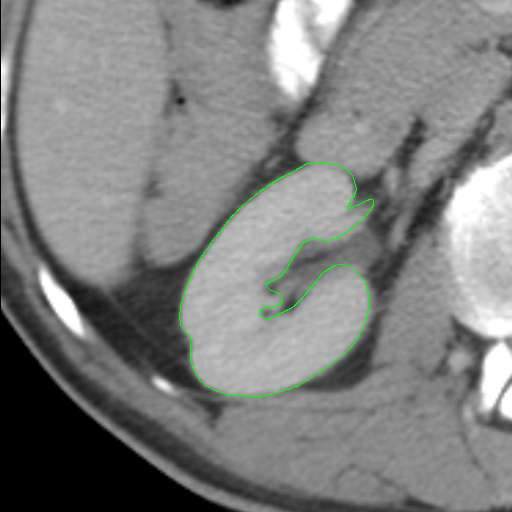
\includegraphics[height=6cm]{appendixval/appendixval-lassotool-before.png}\hspace{8mm}}%
	%
	\hspace{4mm}%
	%
	\subfigure[After evaluating the selection]
	{\hspace{8mm}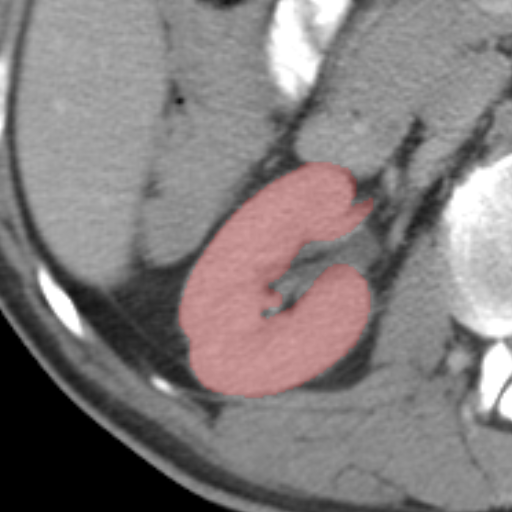
\includegraphics[height=6cm]{appendixval/appendixval-lassotool-after.png}\hspace{8mm}}%
\caption{The lasso tool being used to draw round a kidney}
\label{fig:appendixval-lassotool}
\end{stusubfig}
%---

%~~~~~~~~~~~~~~~~~~~~~~~~~~~~~~~~~~~~~~~~~~~~~~~~
\subsubsection{Line Loop Tool}
%~~~~~~~~~~~~~~~~~~~~~~~~~~~~~~~~~~~~~~~~~~~~~~~~

%---
\begin{stusubfig}{p}
	\subfigure[Before evaluating the selection]
	{\hspace{8mm}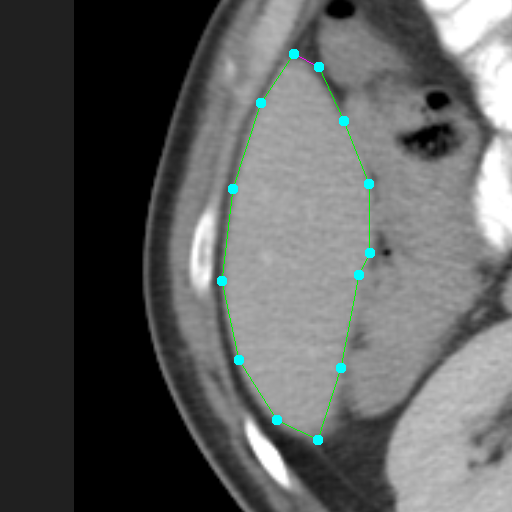
\includegraphics[height=6cm]{appendixval/appendixval-linelooptool-before.png}\hspace{8mm}}%
	%
	\hspace{4mm}%
	%
	\subfigure[After evaluating the selection]
	{\hspace{8mm}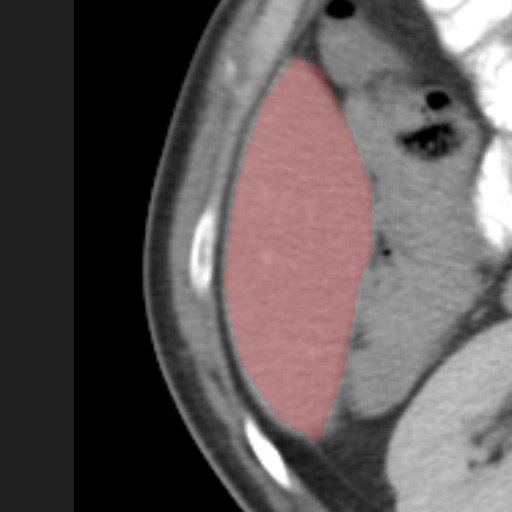
\includegraphics[height=6cm]{appendixval/appendixval-linelooptool-after.png}\hspace{8mm}}%
\caption{The line loop tool being used to draw round a liver}
\label{fig:appendixval-linelooptool}
\end{stusubfig}
%---

The line loop tool is also straightforward in principle -- all that is really necessary is to specify that it is a multi-click tool, and then add the points clicked to the list of drawn locations in its \texttt{mouse_pressed()} method -- but in practice, the tool can be made substantially more usable with a few simple improvements.

Rather than always adding a new point when the user presses the mouse, we first check to see if they are clicking near to an existing point. If so, we `grab' the point, and allow the user to drag it around in \texttt{mouse_dragged()}. If not, we add a new point as usual.

Rendering must also be improved for this to work well -- instead of just rendering the polyline, we also render the individual points as large circular handles (see Figure~\ref{fig:appendixval-linelooptool}(a)). This makes it easier for users to see where they need to click to drag the points around. The code to implement the line loop tool is shown in Listing~\ref{code:appendixval-lineloopdrawingtool}.

%---
\begin{stulisting}[p]
\caption{The LineLoopDrawingTool class}
\label{code:appendixval-lineloopdrawingtool}
\lstinputlisting[style=Default,language=C++]{appendixval/appendixval-lineloopdrawingtool.lst}
\end{stulisting}
%---

\newpage

%################################################
\subsection{GUI Integration}
\label{subsec:appendixval-integration}
%################################################

In \emph{millipede}, the interactions between the drawing tools and the rest of the application are handled in a class called \texttt{DICOMCanvas}, which represents a canvas that displays CT scans. There are two pieces of code necessary -- (a) the canvas's mouse handlers, which process the user's input, forward it to the current drawing tool as necessary and decide when the user has finished drawing (see Listing~\ref{code:appendixval-mousehandlers}), and (b) the \texttt{finish_drawing()} method, which is called by the mouse handlers to rasterize the current drawing, project the rasterized drawing into 3D, and modify the partition forest selection as necessary (see Listing~\ref{code:appendixval-finishdrawing}).

The mouse handlers are fairly straightforward, but there are a few observations that need to be made in order to fully understand them:
%
\begin{enumerate}

\item The \texttt{pixels_to_coords()} method converts from on-screen pixel coordinates to image volume coordinates.
\item The \texttt{within_image_bounds()} method checks whether or not the specified point in pixel coordinates is within the bounds of the image as rendered on the screen.
\item The \texttt{clamp_to_image_bounds()} method clamps a point in pixel coordinates to the bounds of the image as rendered on the screen.

\end{enumerate}
%
Pressing the left mouse button down triggers \texttt{OnLeftDown()}, which first checks that there is a valid partition forest and current drawing tool, and that the mouse press was within the image bounds. If so, it calculates the image volume location of the mouse press, and forwards both that and the pixel location to the current drawing tool. If the tool is an instantaneous one, it then additionally invokes \texttt{finish_drawing()}.

Moving the mouse triggers \texttt{OnMouseMotion()}, which checks whether the left mouse button is down and, if it is, alerts non-instantaneous tools that the mouse is being dragged. The actual location of the drag is clamped to the on-screen bounds of the image, since it doesn't make sense to try and select things outside the image volume.

Letting go of the left mouse button triggers \texttt{OnLeftUp()}, which alerts the tool that the mouse has been released if a drawing is currently in progress (otherwise, the event is ignored). It also invokes \texttt{finish_drawing()} unless the tool is a multi-click one (in which case there is potentially more input to come).

Letting go of the right mouse button triggers \texttt{OnRightUp()}, which is used to finalize multi-click drawings. Moving the mouse outside the window triggers \texttt{OnLeaveWindow()}, which simply resets the current drawing tool.

The \texttt{finish_drawing()} method itself first invokes \texttt{selected_positions()} on the current drawing tool in order to rasterize the drawing. The rasterization produces a std::vector of 2D image coordinates, which are projected into 3D in a manner that depends on which slice is currently being viewed. As an example, if coronal (X-Z) slices were being viewed, with the current value of $y$ (i.e.~the current coronal slice number) being $23$, then the 2D image coordinates $(x,z)$ would be projected into 3D as $(x,23,z)$. Each projected image coordinate is used to look up a leaf in the lowest layer of the partition forest, and a unique set of such leaves is formed. Next, the unique leaves are used to initialise a partition forest selection -- depending on what keys the user is holding down, this is then either used to augment the current selection, subtract from it, or replace it. Finally, the current drawing tool is reset, ready for the user to start a new drawing.

%---
\begin{stulisting}[p]
\caption{The implementation of the DICOMCanvas mouse handlers}
\label{code:appendixval-mousehandlers}
\lstinputlisting[style=Default]{appendixval/appendixval-mousehandlers.lst}
\end{stulisting}
%---

%---
\begin{stulisting}[p]
\caption{The implementation of DICOMCanvas::finish_drawing()}
\label{code:appendixval-finishdrawing}
\lstinputlisting[style=Default]{appendixval/appendixval-finishdrawing.lst}
\end{stulisting}
%---

\newpage

%##################################################################################################
\section{Feature Comparisons}
%##################################################################################################

TODO
